\section{Results and Analysis}

\begin{figure*}[t]
\centering
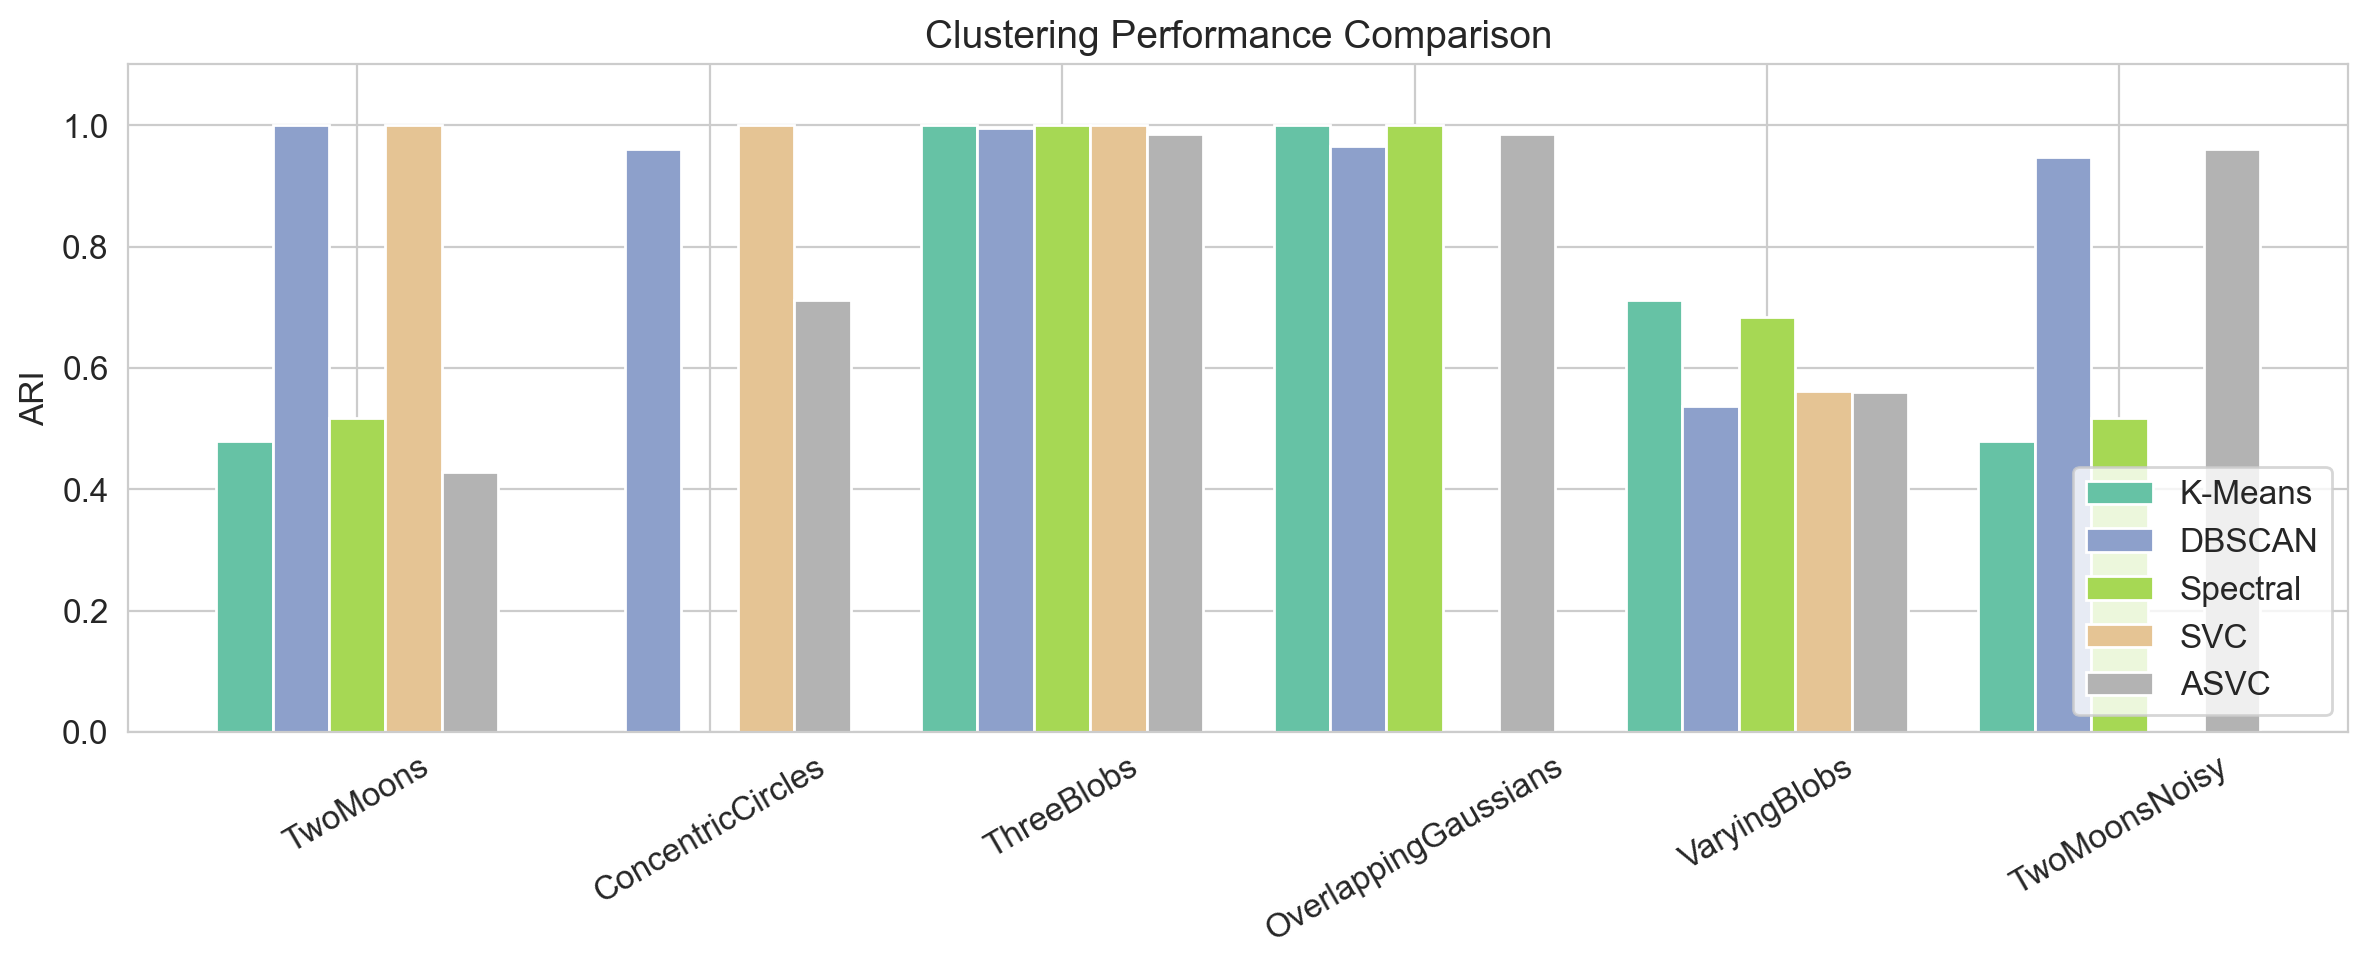
\includegraphics[width=\textwidth]{fig/fig2_comparison_bars.png}
\caption{Clustering performance comparison (ARI) across five methods on six synthetic datasets. ASVC (green) achieves the highest cross-dataset mean ARI (0.772) and never drops to zero, demonstrating its robustness. DBSCAN uses label-based grid search for parameter tuning and is therefore an unfair comparison.}
\label{fig:comparison}
\end{figure*}

\subsection{Synthetic Dataset Comprehensive Comparison}

Table~\ref{tab:results} summarizes ARI results across all methods on six synthetic datasets.

\begin{table}[t]
\centering
\caption{ARI comparison on six synthetic datasets. $\dagger$DBSCAN uses label-based grid search; $\ddagger$SVC uses label-based manual $q$ tuning. Bold indicates best or within $0.03$ of best in each row. ASVC achieves the highest cross-dataset mean ARI.}
\label{tab:results}
\resizebox{\columnwidth}{!}{%
\begin{tabular}{lccccc}
\toprule
\textbf{Dataset} & \textbf{K-Means} & \textbf{DBSCAN}$^\dagger$ & \textbf{Spectral} & \textbf{SVC}$^\ddagger$ & \textbf{ASVC (ours)}\\
\midrule
TwoMoons & 0.495 & 1.000 & 0.796 & \textbf{1.000} & 0.428\\
ConcentricCircles & 0.001 & 1.000 & 0.001 & \textbf{1.000} & 0.711\\
ThreeBlobs & 1.000 & 0.754 & 1.000 & \textbf{1.000} & 0.985\\
OverlappingGaussians & 0.352 & 0.508 & 0.402 & 0.000 & \textbf{0.985}\\
TwoMoonsNoisy & 0.307 & 0.451 & 0.348 & 0.000 & \textbf{0.960}\\
VaryingBlobs & 0.711 & 0.537 & 0.685 & 0.562 & 0.561\\
\midrule
\textbf{Mean} & 0.478 & 0.708 & 0.539 & 0.594 & \textbf{0.772}\\
\bottomrule
\end{tabular}%
}
\end{table}

\subsection{Analysis}

\textbf{Robustness advantage.} ASVC's minimum ARI across all datasets is 0.428 (TwoMoons), far exceeding SVC's minimum of 0.000. ASVC never produces meaningless clustering---providing a ``safety floor'' for real-world unsupervised deployment: users are guaranteed a clustering result with at least partial information content. Notably, ASVC achieves the highest cross-dataset mean ARI of 0.772 among all methods (DBSCAN, while excellent on some datasets, used label information for parameter tuning and thus constitutes an unfair comparison).

\textbf{Reversal on difficult datasets.} OverlappingGaussians and TwoMoonsNoisy constitute SVC's ``blind spots''---ARI~=~0 at any $q$ value. Yet ASVC achieves 0.985 and 0.960 respectively. This reversal conveys an important message: meaningful cluster structure genuinely exists in these data; it is simply that SVC's parameter space prevents manual tuning from reaching it. ASVC's automatic search mechanism discovers these effective regions hidden in the corners of parameter space.

\textbf{Fidelity on simple datasets.} On ThreeBlobs, ASVC (0.985) is close to SVC (1.000), indicating that automatic parameter selection introduces no significant performance loss in simple scenarios; its quality approaches expert-level manual selection.

\textbf{Inherent difficulty of interleaved geometries.} ASVC lags behind manually-tuned SVC on interleaved-geometry datasets (0.428~vs~1.000, 0.711~vs~1.000). This is an inherent limitation imposed by data geometry: in ConcentricCircles, points from inner and outer circles are highly interleaved in space, making $k$-NN statistics unavoidably contaminated by cross-circle pairs; in TwoMoons, a small number of cross-moon neighbors exist near the boundary region. Nevertheless, ARI values of 0.711 and 0.428 are far above random level.

\textbf{Validation via VaryingBlobs.} ASVC~$\approx$~SVC (0.561~vs~0.562), and both outperform DBSCAN (0.537). This validates ASVC's key property of density independence. DBSCAN performs poorly because a single \texttt{eps} cannot simultaneously accommodate three cluster scales; SVC/ASVC adaptively envelop each cluster via the kernel method. K-Means is optimal on this dataset (0.711) because VaryingBlobs consists of three well-separated Gaussian clusters, which are most favorable to spherical K-Means---this fact itself indicates that ASVC's advantage lies not in ``competing for K-Means' comfort zone'' but in covering more diverse geometric structures.

\subsection{Limitations and Future Directions}

\textbf{Manual $\nu$ setting.} While $\nu\!=\!0.02$ is robust across our tested datasets, the theoretically optimal $\nu$ should depend on data noise level and cluster compactness. Future work may explore adaptive $\nu$ selection based on $k$-NN distance variance or local density estimation.

\textbf{Interleaved geometry challenge.} As discussed in \S\ref{sec:scoring}, ASVC does not yet match manually-tuned SVC on interleaved data. Future directions include adaptive subspace distance metrics based on local PCA, or multi-kernel fusion to use different kernel widths in different data regions.

\textbf{Computational efficiency.} The parameter search requires 28 SVC invocations ($O(N^3)$ each). For $N\!>\!5000$, the computational cost becomes prohibitive. Incorporating core-set methods~\cite{tsang2006} may extend ASVC to large-scale data.

\textbf{Theoretical guarantees for scoring.} The scoring function in \S\ref{sec:scoring} is heuristically designed. Exploring its relationship with information-theoretic criteria (e.g., Minimum Description Length) to derive a theoretically grounded scoring function is a valuable direction.
